\documentclass{article}
\usepackage{graphicx}
\usepackage{amsmath} % For math formatting


\begin{document}

\title{Fall-2023 5304 PrEx04}
\author{Wan}
\date{\today}
\maketitle

\noindent
This exercise is related to LecN5 and LecN6.

\section{Q1: True or False}
\subsection{a: If A and B are SPD then A+B is also SPD}
True. Using the operation property of inner product\\
$\left\langle (A+B)u,u\right\rangle = 
\left\langle Au,u\right\rangle + \left\langle Bu,u\right\rangle > 0
$

\subsection{b: When A is SPD then its inverse is also SPD}
True. There are 2 ways to show.\\
\\
Way1: 2nd part def of SPD and property of eigen val.\\
\\
\noindent
A matrix is SPD if it is symmetric and its eigenvalues are positive.
Then, use the fact that the eigenvalues of $A^{-1}$ are (1/eigenvalues of A).\\
\\
Way2: Use 1st part def of SPD and the property of inner product.\\
\\
\noindent
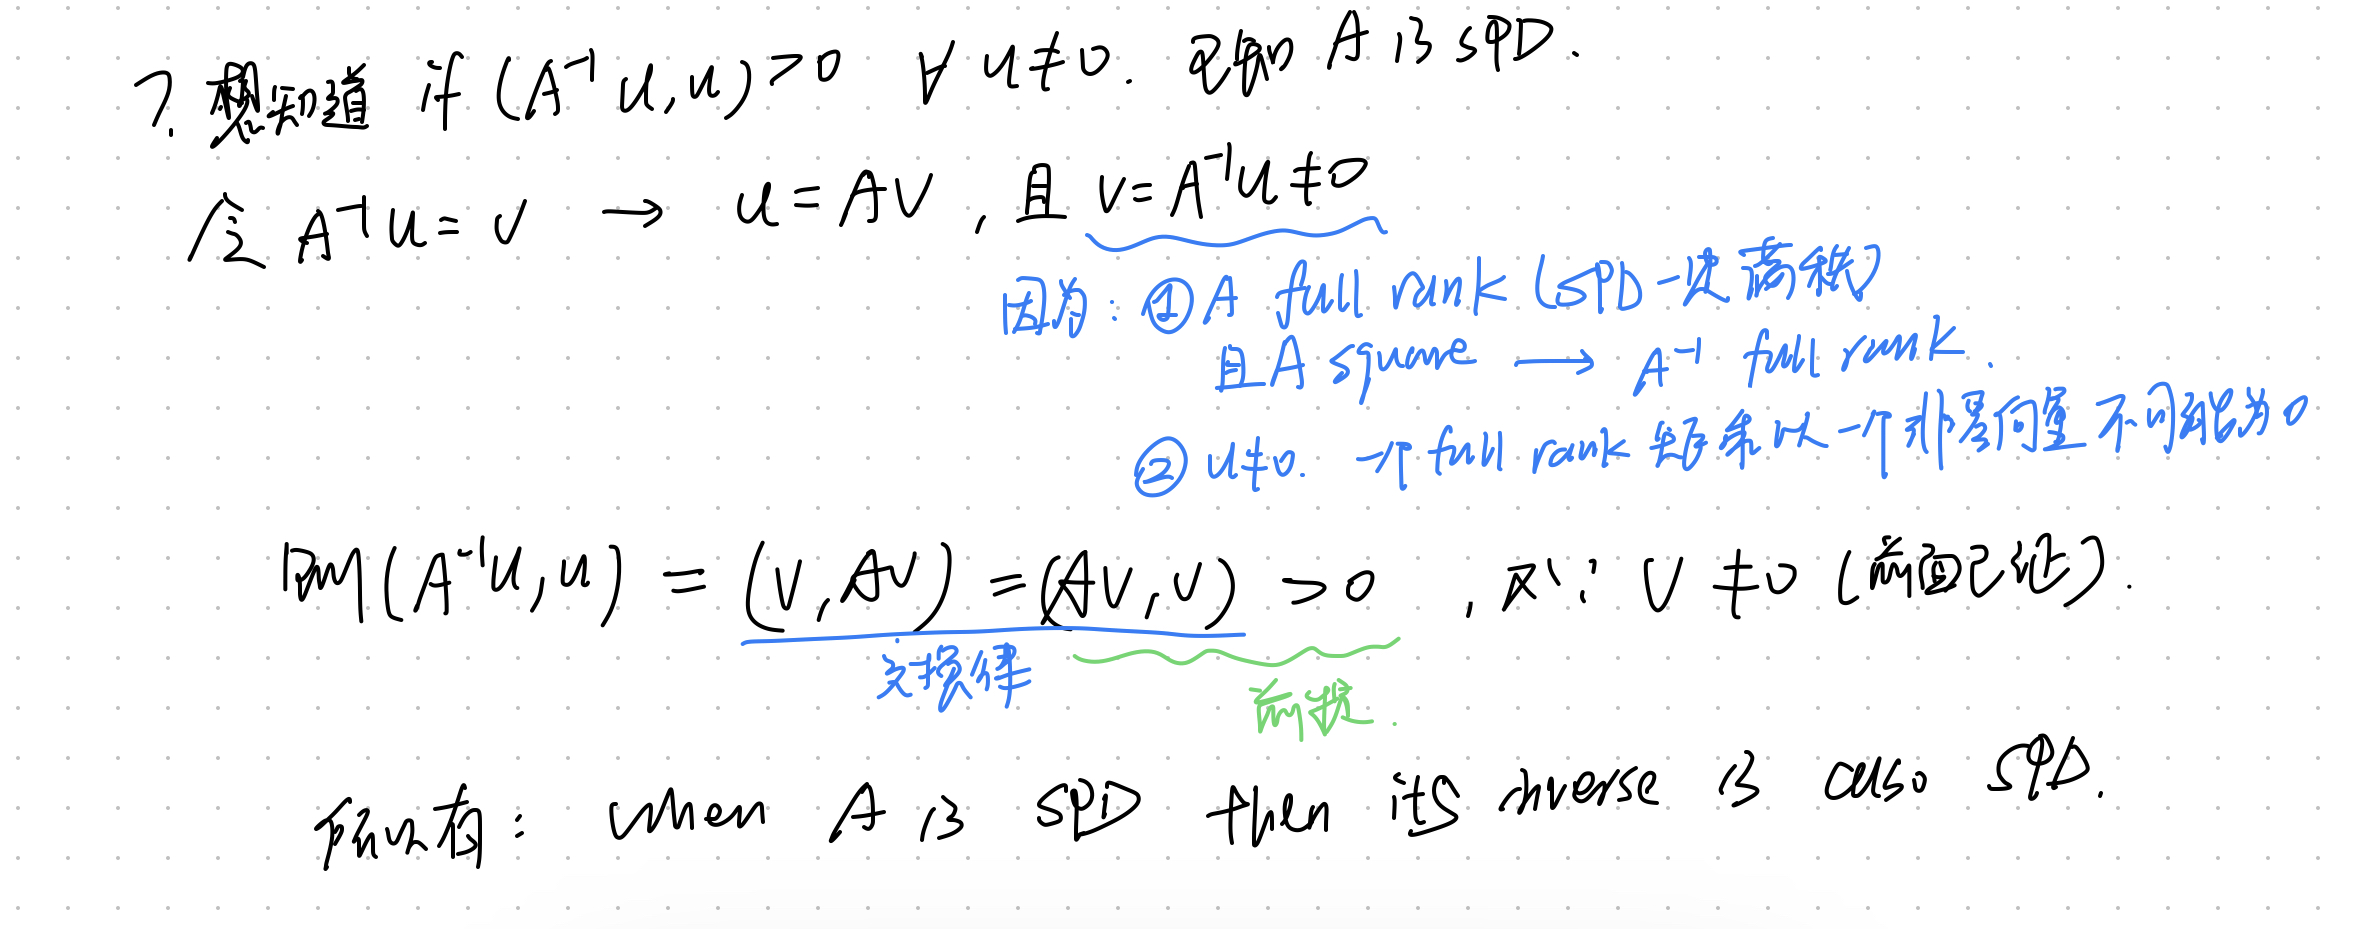
\includegraphics[width=1\linewidth]{pr4-1.jpeg}

\subsection{c: If A = $GG^T$ is the Cholesky factorization of A, what can you say about det(A)}
det(A) = det($GG^T$) = det(G)det($G^T$) = det(G)det(G) = det(G)$^2$\\
just the square of the product of the diagonal entries of G.\\
Notes: A can do GGT implying that A is SPD.

\subsection{d: $X$ is a full-rank $n \times k$ iff $X^TX$ is SPD}
True.\\
\\
Direction 1 (2 ways): If $X$ is a full-rank $n \times k$ matrix, then $X^TX$ is SPD.\\
Way1:\\
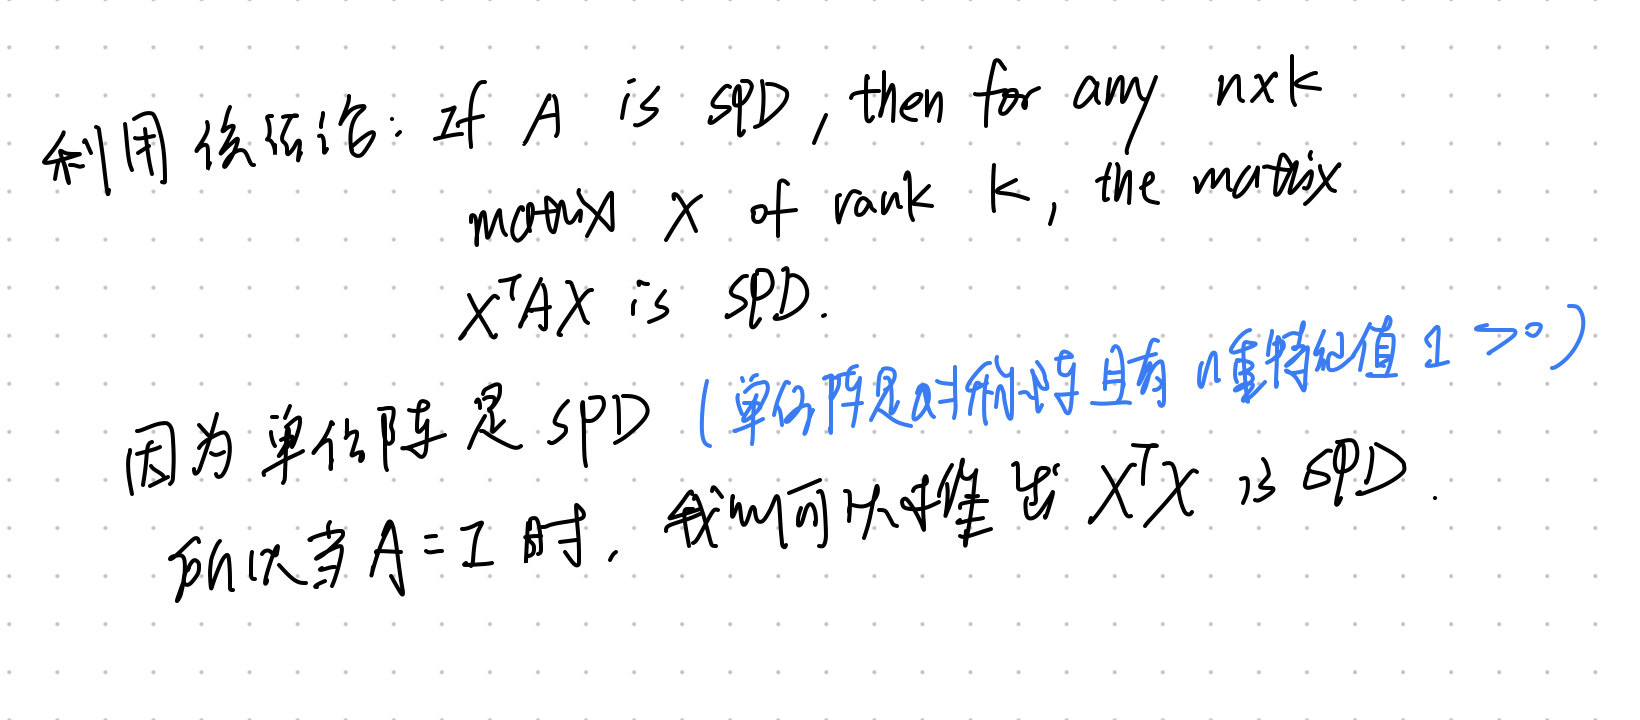
\includegraphics[width=1\linewidth]{pr4-2}

\noindent
Way2: Use property of inner product.\\
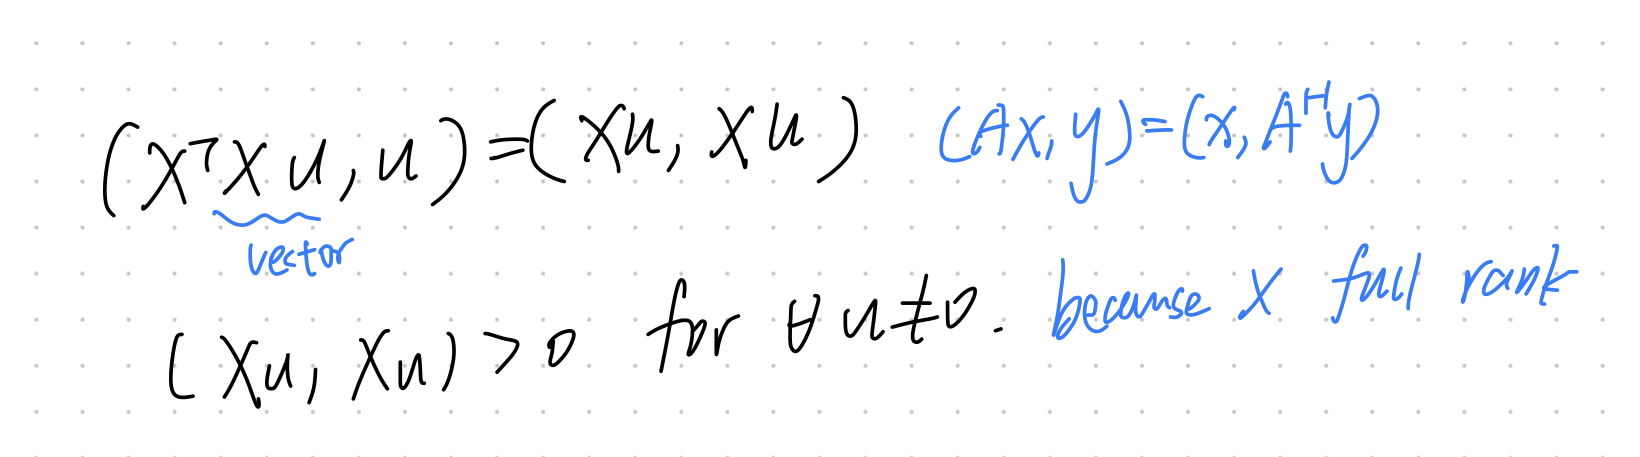
\includegraphics[width=1\linewidth]{pr4-3}

\medskip
\noindent
Direction 2: If $X^TX$ is SPD, then $X$ is a full-rank $n \times k$ matrix.\\
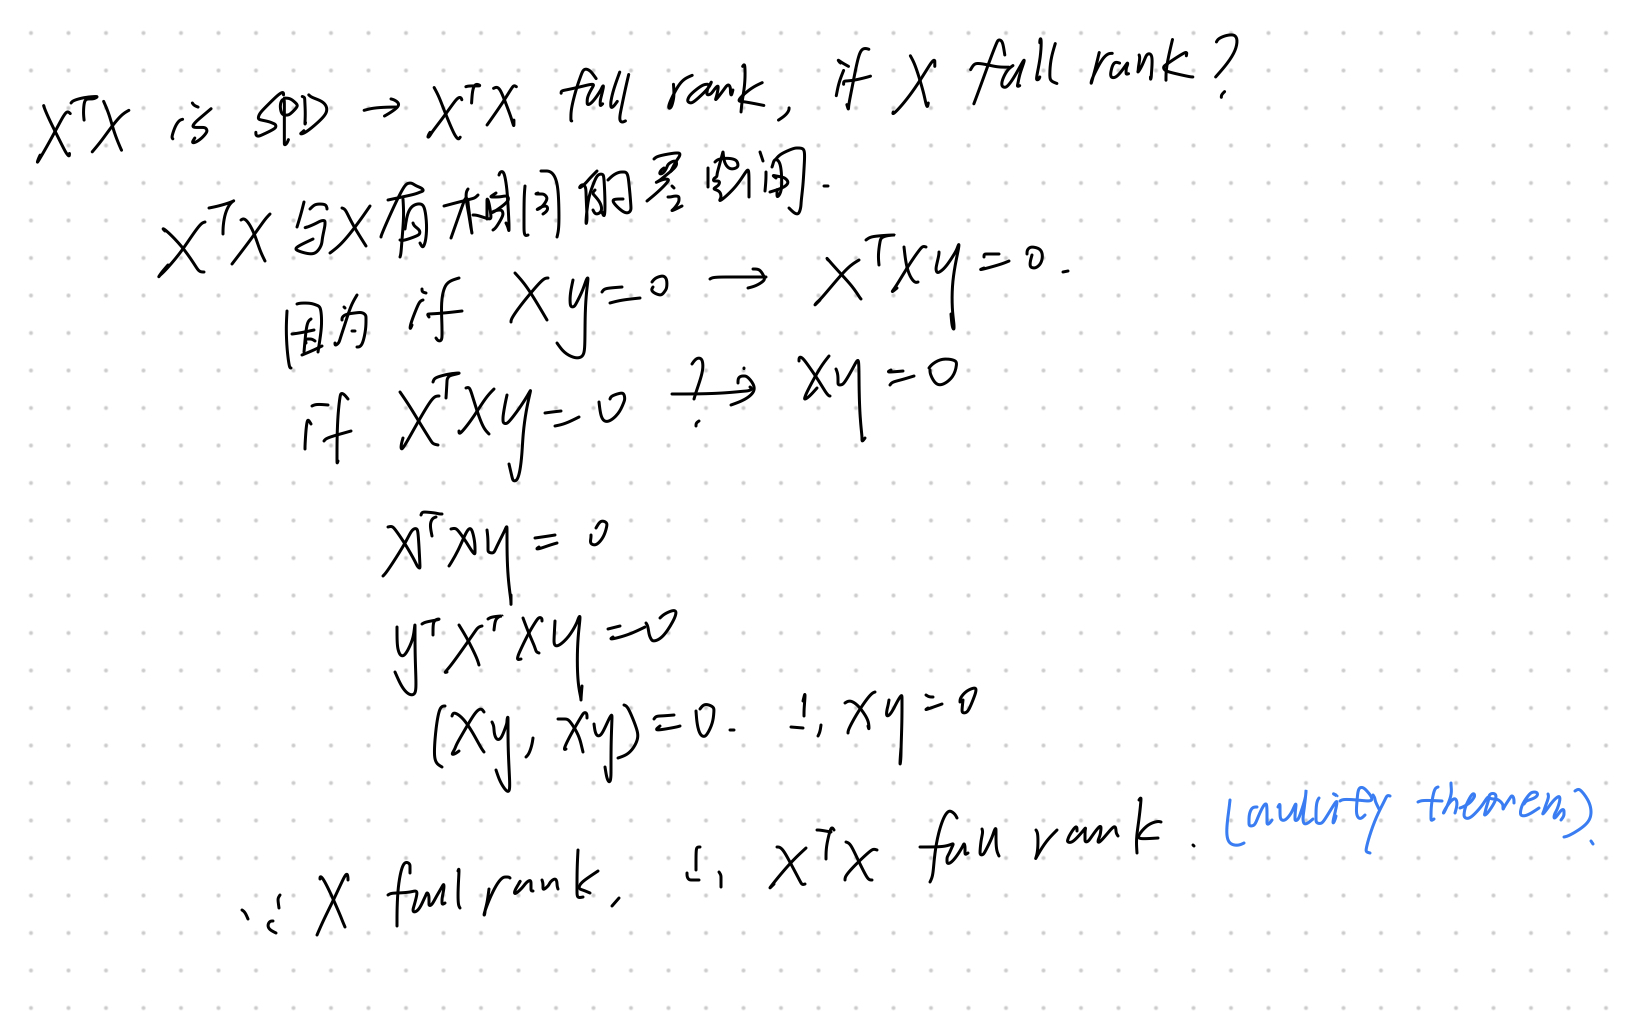
\includegraphics[width=1\linewidth]{pr4-4}


\subsection{e: The Cholesky factorization of $A$ exists iff A is SPD.}
True.\\
\\
Direction 1: If A is SPD, then the Cholesky factorization of $A$ exists.\\
This is proved in class.\\

\noindent
Direction 2: If the Cholesky factorization of $A$ exists, then A is SPD.\\
Premise: G and GT always full rank because: \\
\includegraphics[width=1\linewidth]{pr4-5}
Then, We can use the conclusion from d that: if X is a full-rank matrix iff $X^TX$ is SPD.\\
Let X = $G^T$, then $(G^T)^TG^T = GG^T$ is SPD, then $A = GG^T$ is also SPD.\\

\pagebreak
\section{Q2}
\includegraphics[width=1\linewidth]{pr4-6}

\subsection{Find vector v, 2 ways}
\textbf{Way1: tao is 0 and A becomes singular}\\
\includegraphics[width=1\linewidth]{pr4-7}

\noindent
\textbf{Way2: utilize matrix-vector product}\\
\includegraphics[width=1\linewidth]{pr4-8}


\subsection{Deduce lower bound for norm-inf invA and kapa-inf A}
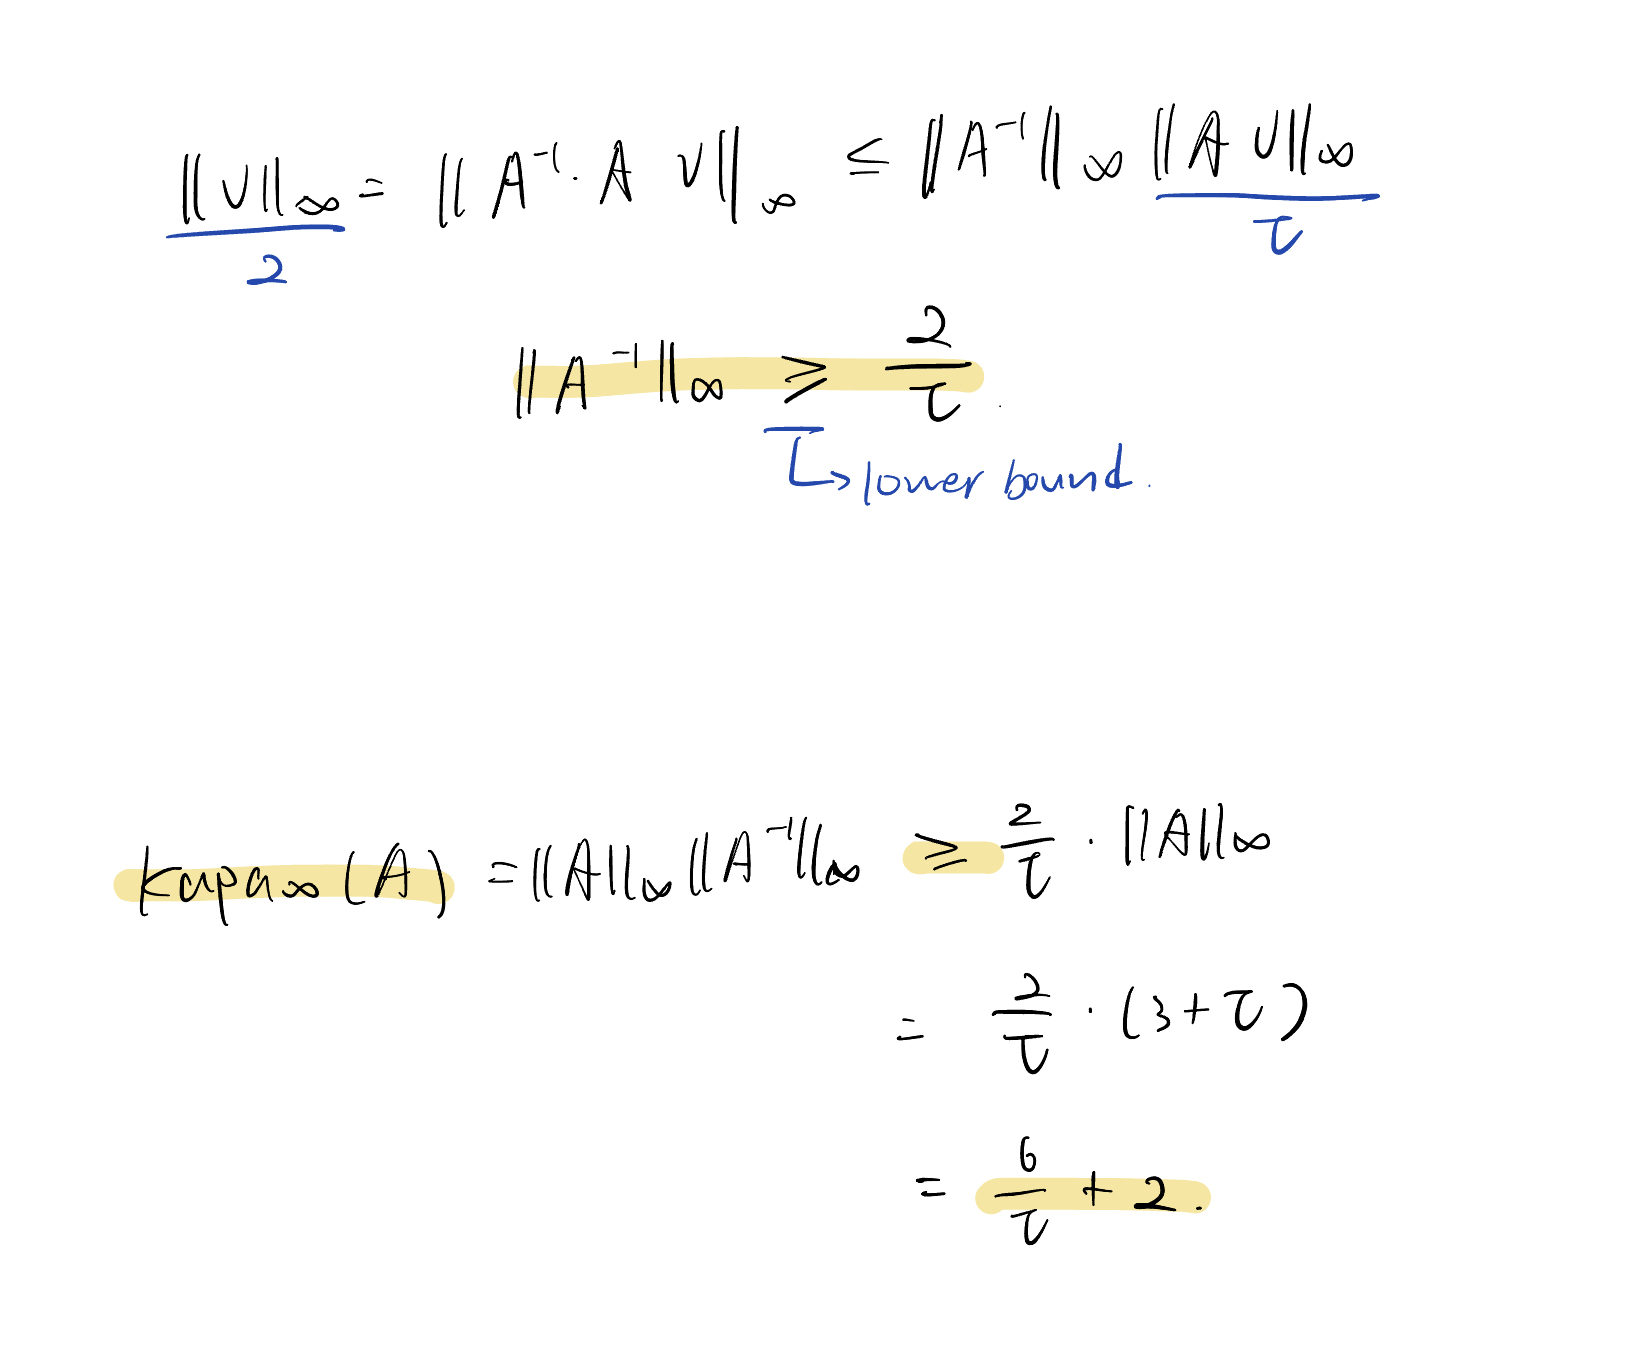
\includegraphics[width=1\linewidth]{pr4-9.jpeg}


\subsection{Calculate kapa-inf A}
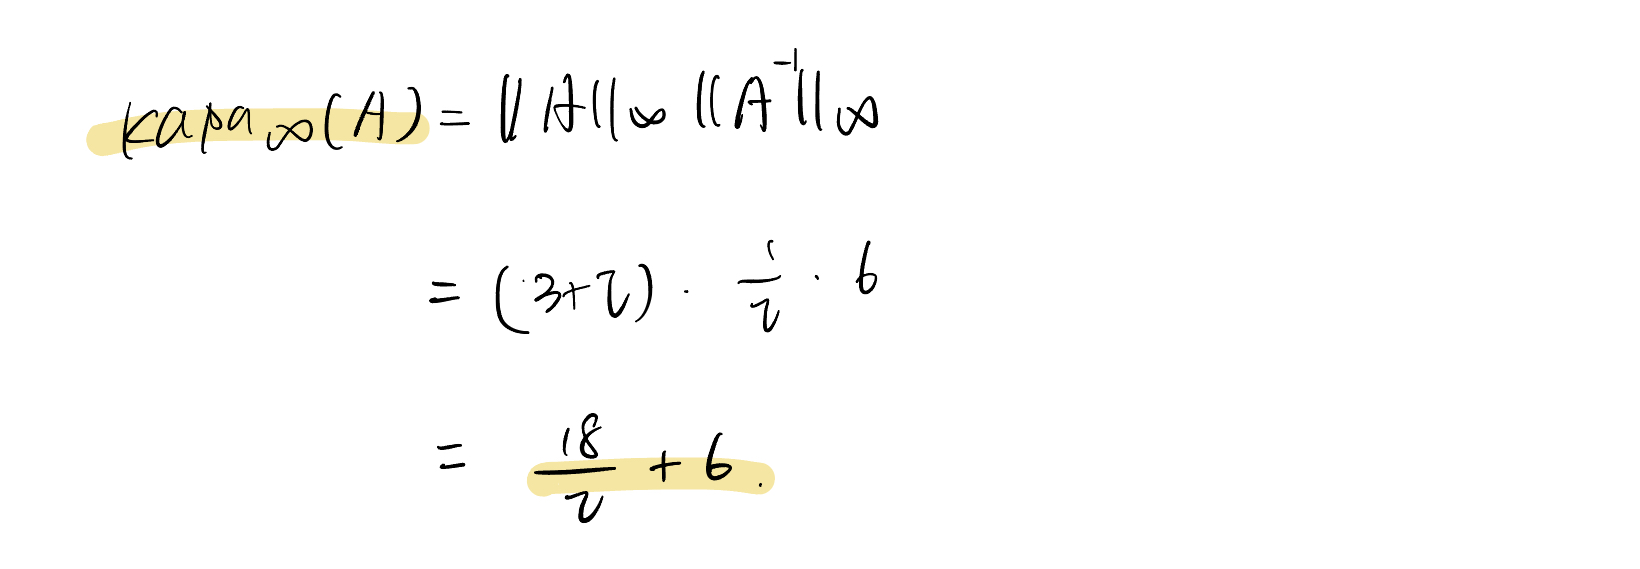
\includegraphics[width=1\linewidth]{pr4-10}

\end{document}